\documentclass[12pt,dvipsnames]{article}
\usepackage[utf8]{inputenc}

\usepackage{microtype}
%\usepackage{charter}
%\usepackage{palatino}
%\usepackage{newcent}
% \usepackage{bookman}
\usepackage{mathpazo}

\usepackage{tikz} % for data flow diagram
\usetikzlibrary{arrows}
\usetikzlibrary{shapes.geometric}
\usetikzlibrary{positioning}
\usetikzlibrary{decorations.text, decorations.shapes, arrows.meta}

% Nice captions.
\usepackage[hang,small,bf]{caption}
\setlength{\captionmargin}{25pt}

\usepackage{xcolor}

\usepackage{hyperref}
\hypersetup{pdfauthor={Adames, Pablo},
			pdftitle={Software Versioning},
			pdfsubject={Software versioning},
			pdfkeywords={versioning}}
\hypersetup{colorlinks,breaklinks,%
            linkcolor=BrickRed,%
            urlcolor=Blue,%
            anchorcolor=Violet,%
            citecolor=MidnightBlue}
            
\title{SoftwareVersioning}
\author{Pablo Adames}
\date{November 11, 2022}

\begin{document}

\maketitle

\section{Introduction}

Software versioning is a convention to keep track of a software product as it goes through its life cycle, from development to deployment and from production to sustainment\cite{Wikipedia_software_version_short}.

In general, versions are unique for every state of the software and follow a sequence to indicate the nature of the change from one state to the next.

Versioning is required for consistency and to facilitate teamwork around writing, building, testing, deploying, selling, and maintaining the product. 


Complex software is made up of multiple inter-operating components. 
An extreme case is a micro-services architecture with the system composed of independent and specialized pieces designed to interact in order to complete a complex task.

The version of the finished product is important for everyone involved. 
The version of the individual components is more important for the developers, testers, and maintainers of the product.

Component version resolution is addressed during the build process.
The most common strategy is to have a component know the minimum (latest) version of the other components it needs, see \ref{fig:dependency-to-build-self}. 
It is also possible to have each component know the list of others that depend on it, see \ref{fig:dependency-to-build-others}.  

\begin{figure}
    \centering
    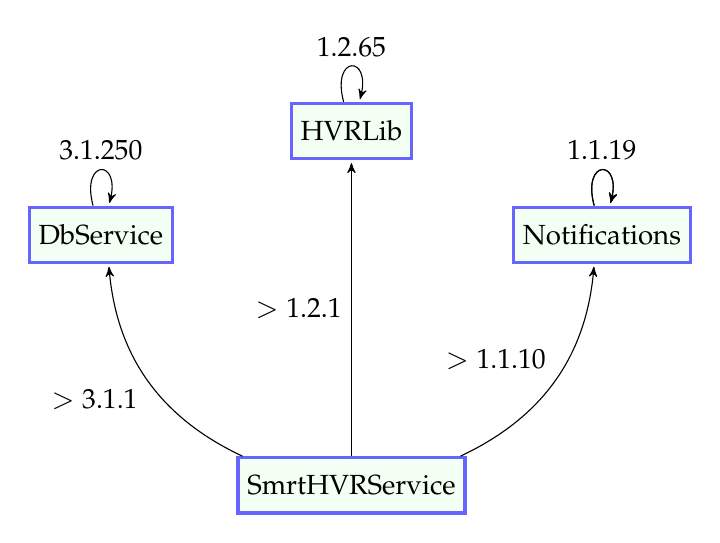
\begin{tikzpicture}[
        rnode/.style={rectangle, draw=blue!60!white, fill=green!5, very thick, minimum size=7mm}, 
        node distance=4.5cm,
        ->,>=stealth',shorten >=1pt,auto
    ]
        \node[rnode] (A) {SmrtHVRService};
        \node[rnode] (B) [above of=A] {HVRLib};
        \node[rnode] (C) [above left of= A]{DbService};
        \node[rnode] (D) [above right of=A] {Notifications};

        \path (A) edge node {$>1.2.1$} (B)
            (A) edge [bend left] node {$>3.1.1$} (C)
            (A) edge [bend right] node {$>1.1.10$} (D)(D) edge [loop above] node {} (D)
            (B) edge [loop above] node {1.2.65} (B)
            (C) edge [loop above] node {3.1.250} (C)
            (D) edge [loop above] node {1.1.19} (D);
    \end{tikzpicture}
  \caption{Fictional example of component dependency resolution where component \textit{SmrtHVRService} requires minimum versions of \textit{DBService} $>$ v3.1.1, \textit{HVRLib} $>$ v1.2.1, and \textit{Notifications} $>$ v1.1.10}
    \label{fig:dependency-to-build-self}
\end{figure}


\begin{figure}
    \centering
    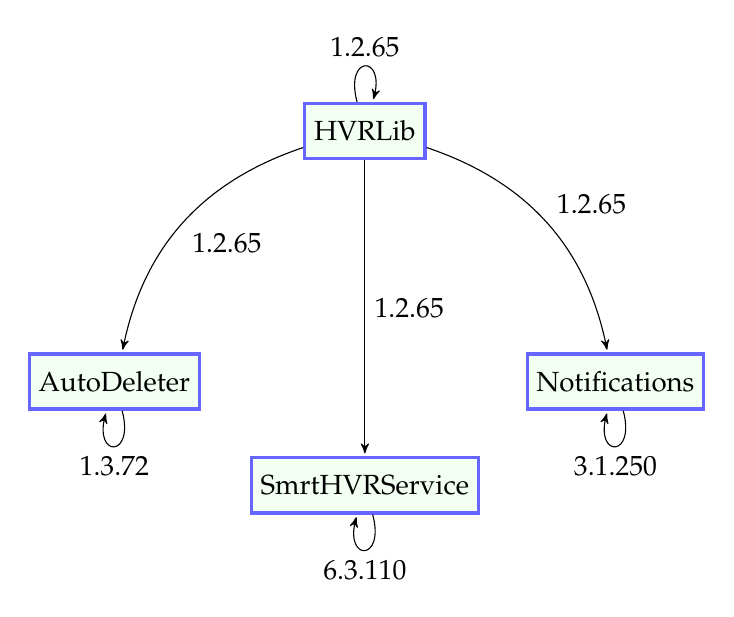
\begin{tikzpicture}[
        rnode/.style={rectangle, draw=blue!60!white, fill=green!5, very thick, minimum size=7mm}, 
        node distance=4.5cm,
        ->,>=stealth',shorten >=1pt,auto
    ]
        \node[rnode] (A) {HVRLib};
        \node[rnode] (B) [below of=A] {SmrtHVRService};
        \node[rnode] (C) [below right of= A]{Notifications};
        \node[rnode] (D) [below left of= A]{AutoDeleter};

        \path (A) edge node {1.2.65} (B)
            (A) edge [bend left] node {1.2.65} (C)
            (A) edge [bend right] node {1.2.65} (D)
            
            (A) edge [loop above] node {1.2.65} (A)
            (B) edge [loop below] node {6.3.110} (B)
            (C) edge [loop below] node {3.1.250} (C)
            (D) edge [loop below] node {1.3.72} (D);
    \end{tikzpicture}
  \caption{Fictional example of component dependency resolution where component \textit{HVRLib} is required to build \textit{Notifications}, \textit{SmrtHVRService}, and \textit{AutoDeleter}}
    \label{fig:dependency-to-build-others}
\end{figure}

The most widely used system is semantic versioning \cite{Wikipedia_software_version}.
It has three parts: major.minor.patch.



\section{Definitions}

\begin{itemize}
    \item CI/CD: continuous integration and continuous deployment 
    \item Pipeline: automated processes to transform source code 
    into software artifacts that can be deployed to computation platforms
    \item Source control or version control: a system to organize and maintain multiple versions of files, usually containing computer language code or configuration.    
    \item Build tools: 
    \item Configuration management:
    \item Monitoring: 
\end{itemize}

% can use a bibliography generated by BibTeX as a .bbl file
% BibTeX documentation can be easily obtained at:
% http://mirror.ctan.org/biblio/bibtex/contrib/doc/
% The IEEEtran BibTeX style support page is at:
% http://www.michaelshell.org/tex/ieeetran/bibtex/
\bibliographystyle{acm}
% argument is your BibTeX string definitions and bibliography database(s)
\bibliography{sources}
%
% <OR> manually copy in the resultant .bbl file
% set second argument of \begin to the number of references
% (used to reserve space for the reference number labels box)
% \begin{thebibliography}{1}

% \bibitem{IEEEhowto:kopka}
% H.~Kopka and P.~W. Daly, \emph{A Guide to \LaTeX}, 3rd~ed.\hskip 1em plus
%   0.5em minus 0.4em\relax Harlow, England: Addison-Wesley, 1999.

% \end{thebibliography}




\end{document}
